% !TeX TS-program = xelatex

\documentclass[10pt]{beamer}

\usetheme[progressbar=frametitle]{metropolis}
\usepackage{appendixnumberbeamer}
\usepackage{pgfplots}
\usepackage{xspace}

\definecolor{links}{HTML}{2A1B81}

\hypersetup{colorlinks,linkcolor=,urlcolor=links}


\newcommand{\themename}{\textbf{\textsc{metropolis}}\xspace}
%\setsansfont[BoldFont={Fira Sans}]{Fira Sans Light}
%\setmonofont{Fira Mono}
%\usepackage[sfdefault]{Fira Sans}

\title{}
\subtitle{}

\author{}

\date{EE/GW meeting, May 25, 2023}

\begin{document}
	
	\maketitle
	
	\begin{frame}{}
		
		Last time: 
		
\includegraphics[width=0.85\textwidth,height=0.85\textwidth]{images/canonical12_result}


\end{frame}


	\begin{frame}{}
	
	Last time: 
	
	\begin{itemize}
		\item Earth terms model $g'(\tau; \bar{\theta}) = 1 - \frac{1}{2} \frac{ H_{ij}q^i q^j }{(1 + \bar{n}\cdot \bar{q}) } \left[ \cos(-\Omega \tau +\Phi_0) \right]$
		\item Zero process noise  $\sigma_p = 0$
		\item No heterodyning
		\item Single noise realisation
		\item Single set of parameters realisation
    \end{itemize}	

\end{frame}



	\begin{frame}{}
	
	This time: 
	
	\begin{itemize}
		\item Earth terms model 
		\item \alert{Non - zero process noise  $\sigma_p \neq 0$} $\checkmark$
		\item \alert{Heterodyning} $\checkmark$
		\item \alert{Multiple noise realisations} $\checkmark$
		\item Single set of parameters realisation
	\end{itemize}	
	
\end{frame}



	\begin{frame}{}
	
	Reminder of "heterodyned" equations
	
	\begin{itemize}
		\item Heterodyne the state: $f \, ' = f - f_{\rm EM}$ 
		\item Heterodyne the measurement: $f \, '_{\rm M}  = f_{\rm M} - f^{\, *}_{\rm EM}$ 
	\end{itemize}
	
	Note the distinction between $ f_{\rm EM}$ and $f^{\, *}_{\rm EM}$
	
	$f_{\rm EM}$ is the exact, true solution parametrised by the unknowns $f_0, \dot{f}_0$. This ``heterodyning" is just a change of variables
	
	$f^{\, *}_{\rm EM}$ is a guess of $f_{\rm EM}$ based on the pulsar ephemeris. It is just to scale the equations - it does not remove any degrees of freedom - we still are estimating $f_0, \dot{f}_0$ optimally!
		
	\begin{equation}
		\frac{df \, '}{dt} = - \gamma f \, '  + \xi 
	\end{equation}

	\begin{eqnarray}
		f \, '_{\rm M} = (1 - X)f \, ' - X f_{\rm EM} + \alert{(f_{\rm EM} - f^{\, *}_{\rm EM})} +  N_{\rm G}
	\end{eqnarray}

	For our case where we have synthetic data we can set $f_{\rm EM} = f^{\, *}_{\rm EM}$. In the general ``real-world" case we cannot - but this is just a scaling, not a  fundamental structure viz. d.o.f
	
	
\end{frame}


	\begin{frame}[label={first_slide}]
	
	
	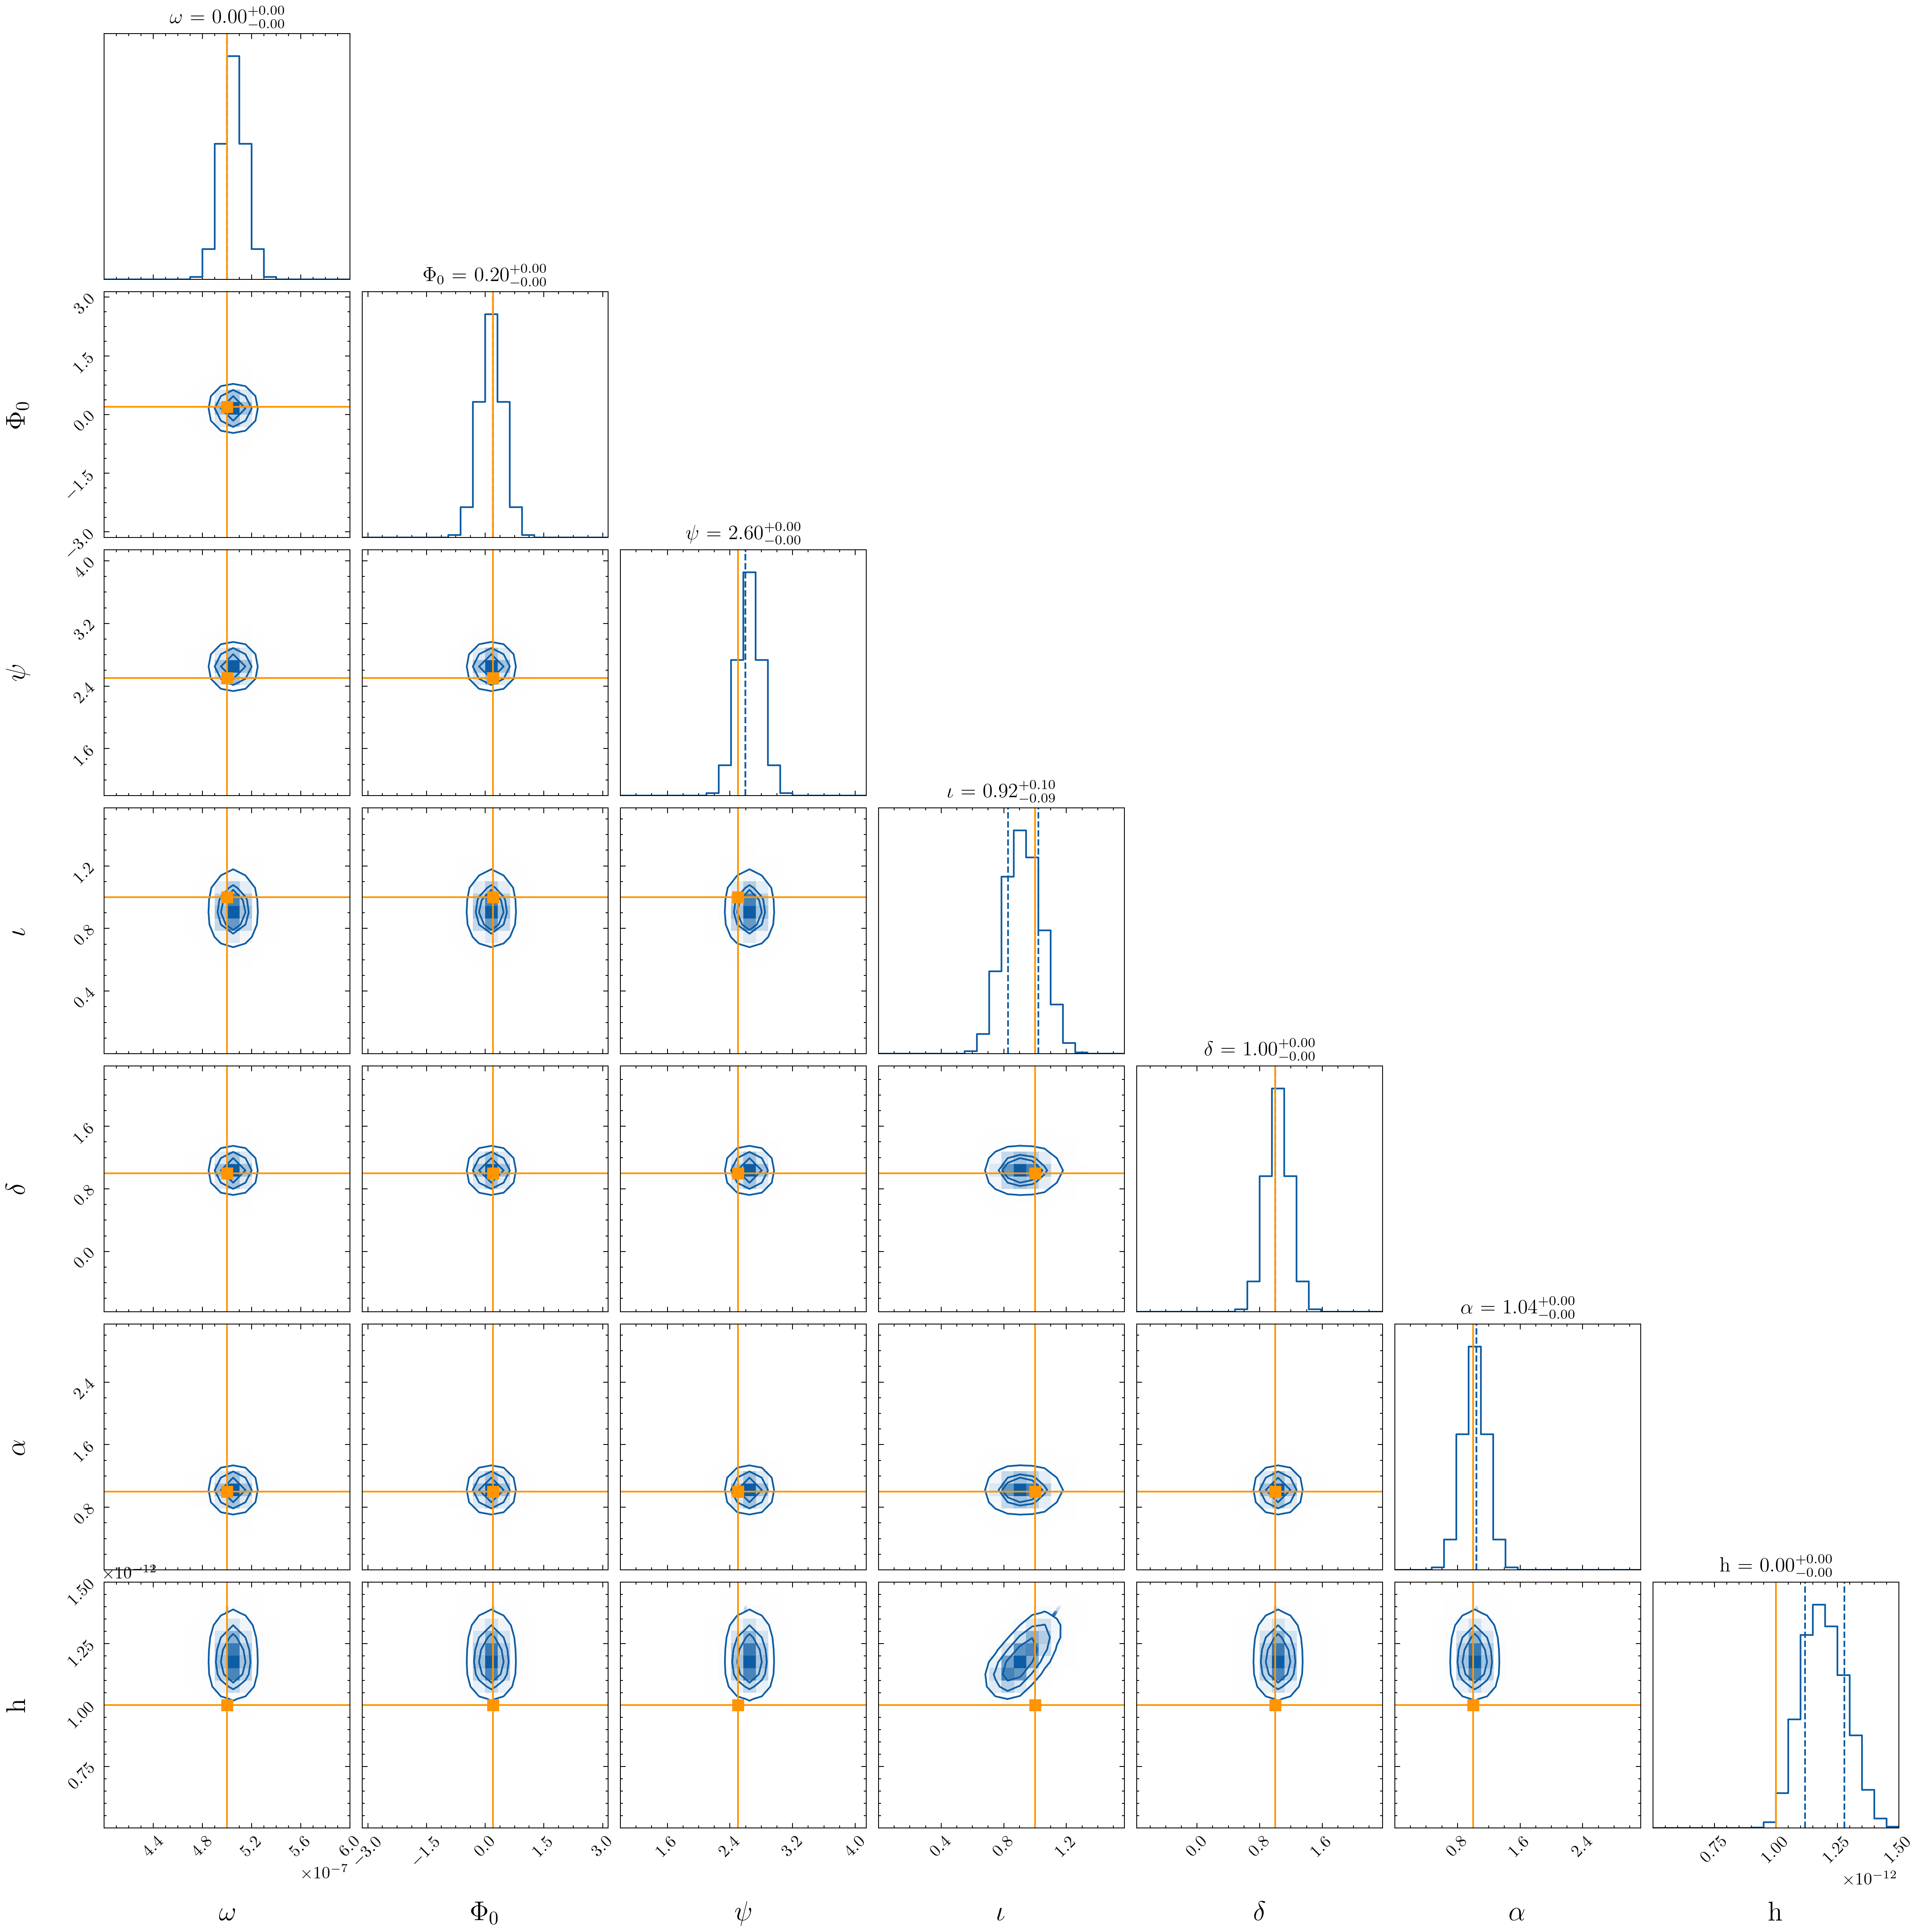
\includegraphics[width=0.85\textwidth,height=0.85\textwidth]{images/1237_broad_GW}
		\only<1>{%
		\tikz[overlay,remember picture]
		\node[fill=white,text=black] at ([xshift=1.5cm,yshift=3.5cm]current page.center){$h = 10^{-12}$, $\sigma_p = \mathcal{U}(10^{-21}, 10^{-19})$};
	}
	\only<1>{%
	\tikz[overlay,remember picture]
	\node[fill=white,text=black] at ([xshift=1.5cm,yshift=3.0cm]current page.center){Heterodyned equations, Full PTA};
	
}
	\only<1>{%
	\tikz[overlay,remember picture]
	\node[fill=white,text=black] at ([xshift=1.5cm,yshift=2.5cm]current page.center){$\bar{\theta}_{\rm GW}$, c.f. Slide \ref{first_slide_noise}};
	
}


	
\end{frame}

	\begin{frame}{}
	
	
	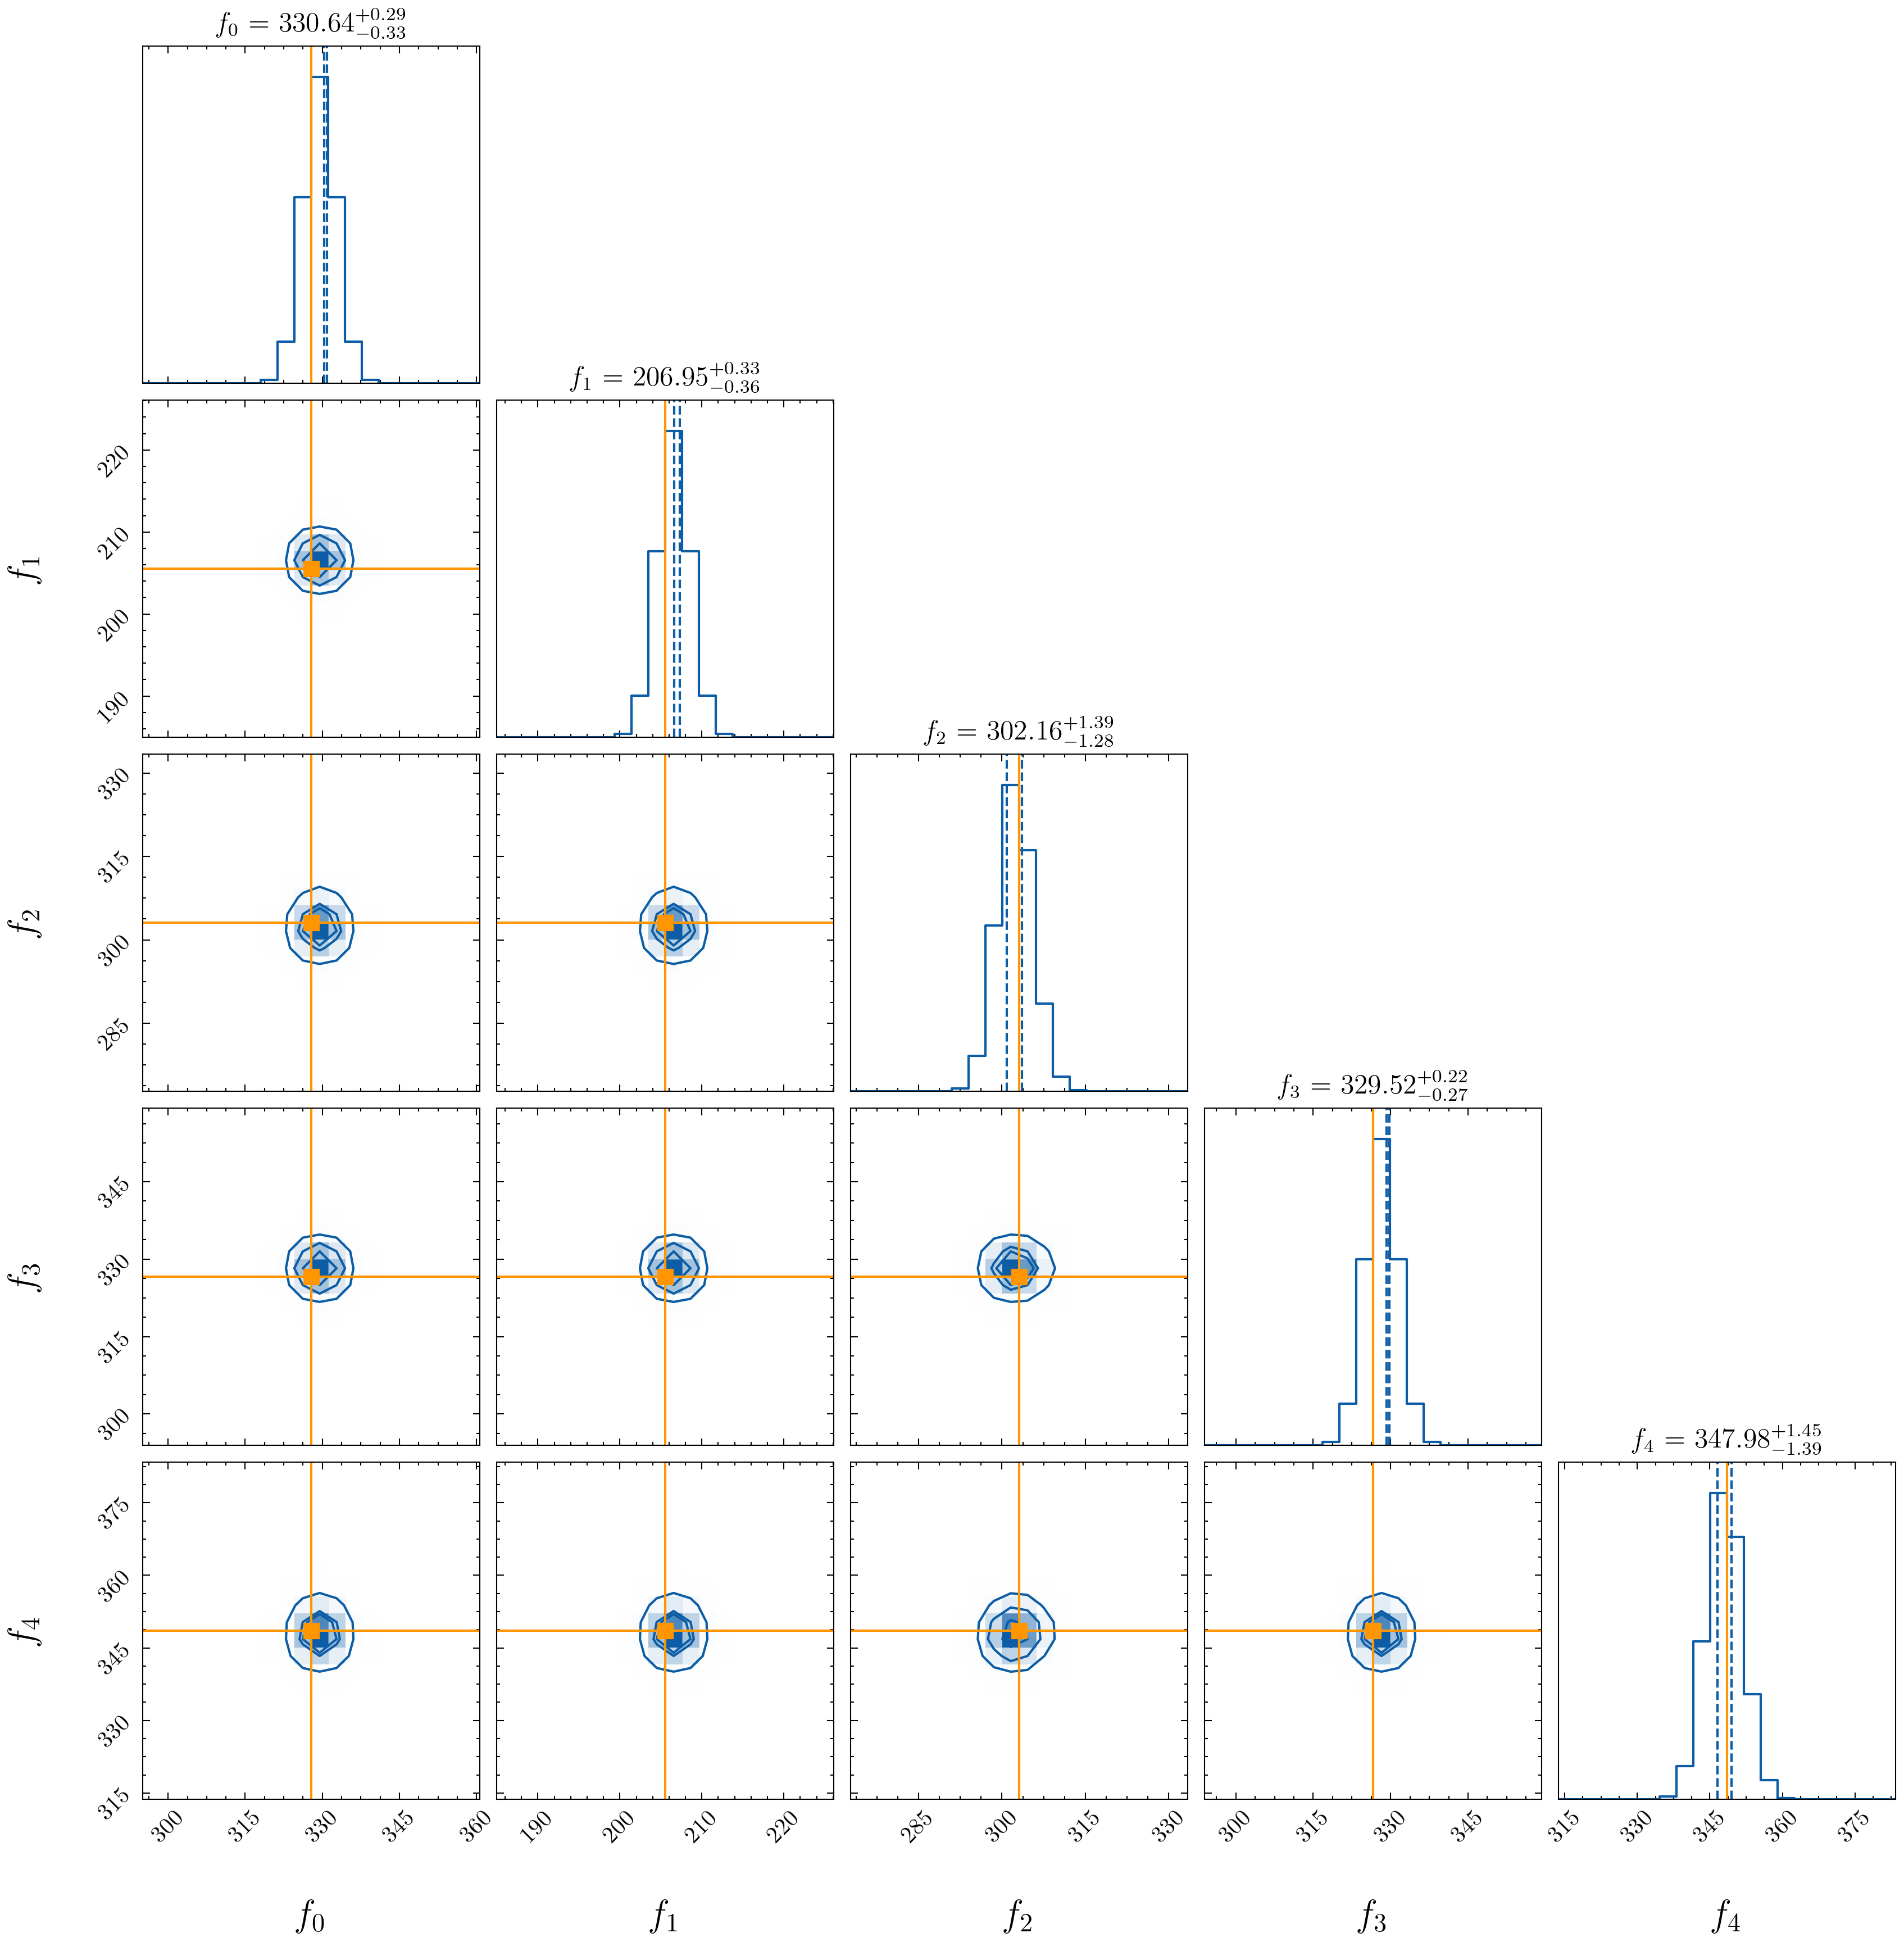
\includegraphics[width=0.85\textwidth,height=0.85\textwidth]{images/1237_broad_f}
	
		\only<1>{%
		\tikz[overlay,remember picture]
		\node[fill=white,text=black] at ([xshift=1.5cm,yshift=3.5cm]current page.center){Slightly deceptive: very tight priors - to discuss};
	}
	
\end{frame}



	\begin{frame}{}
	
	
	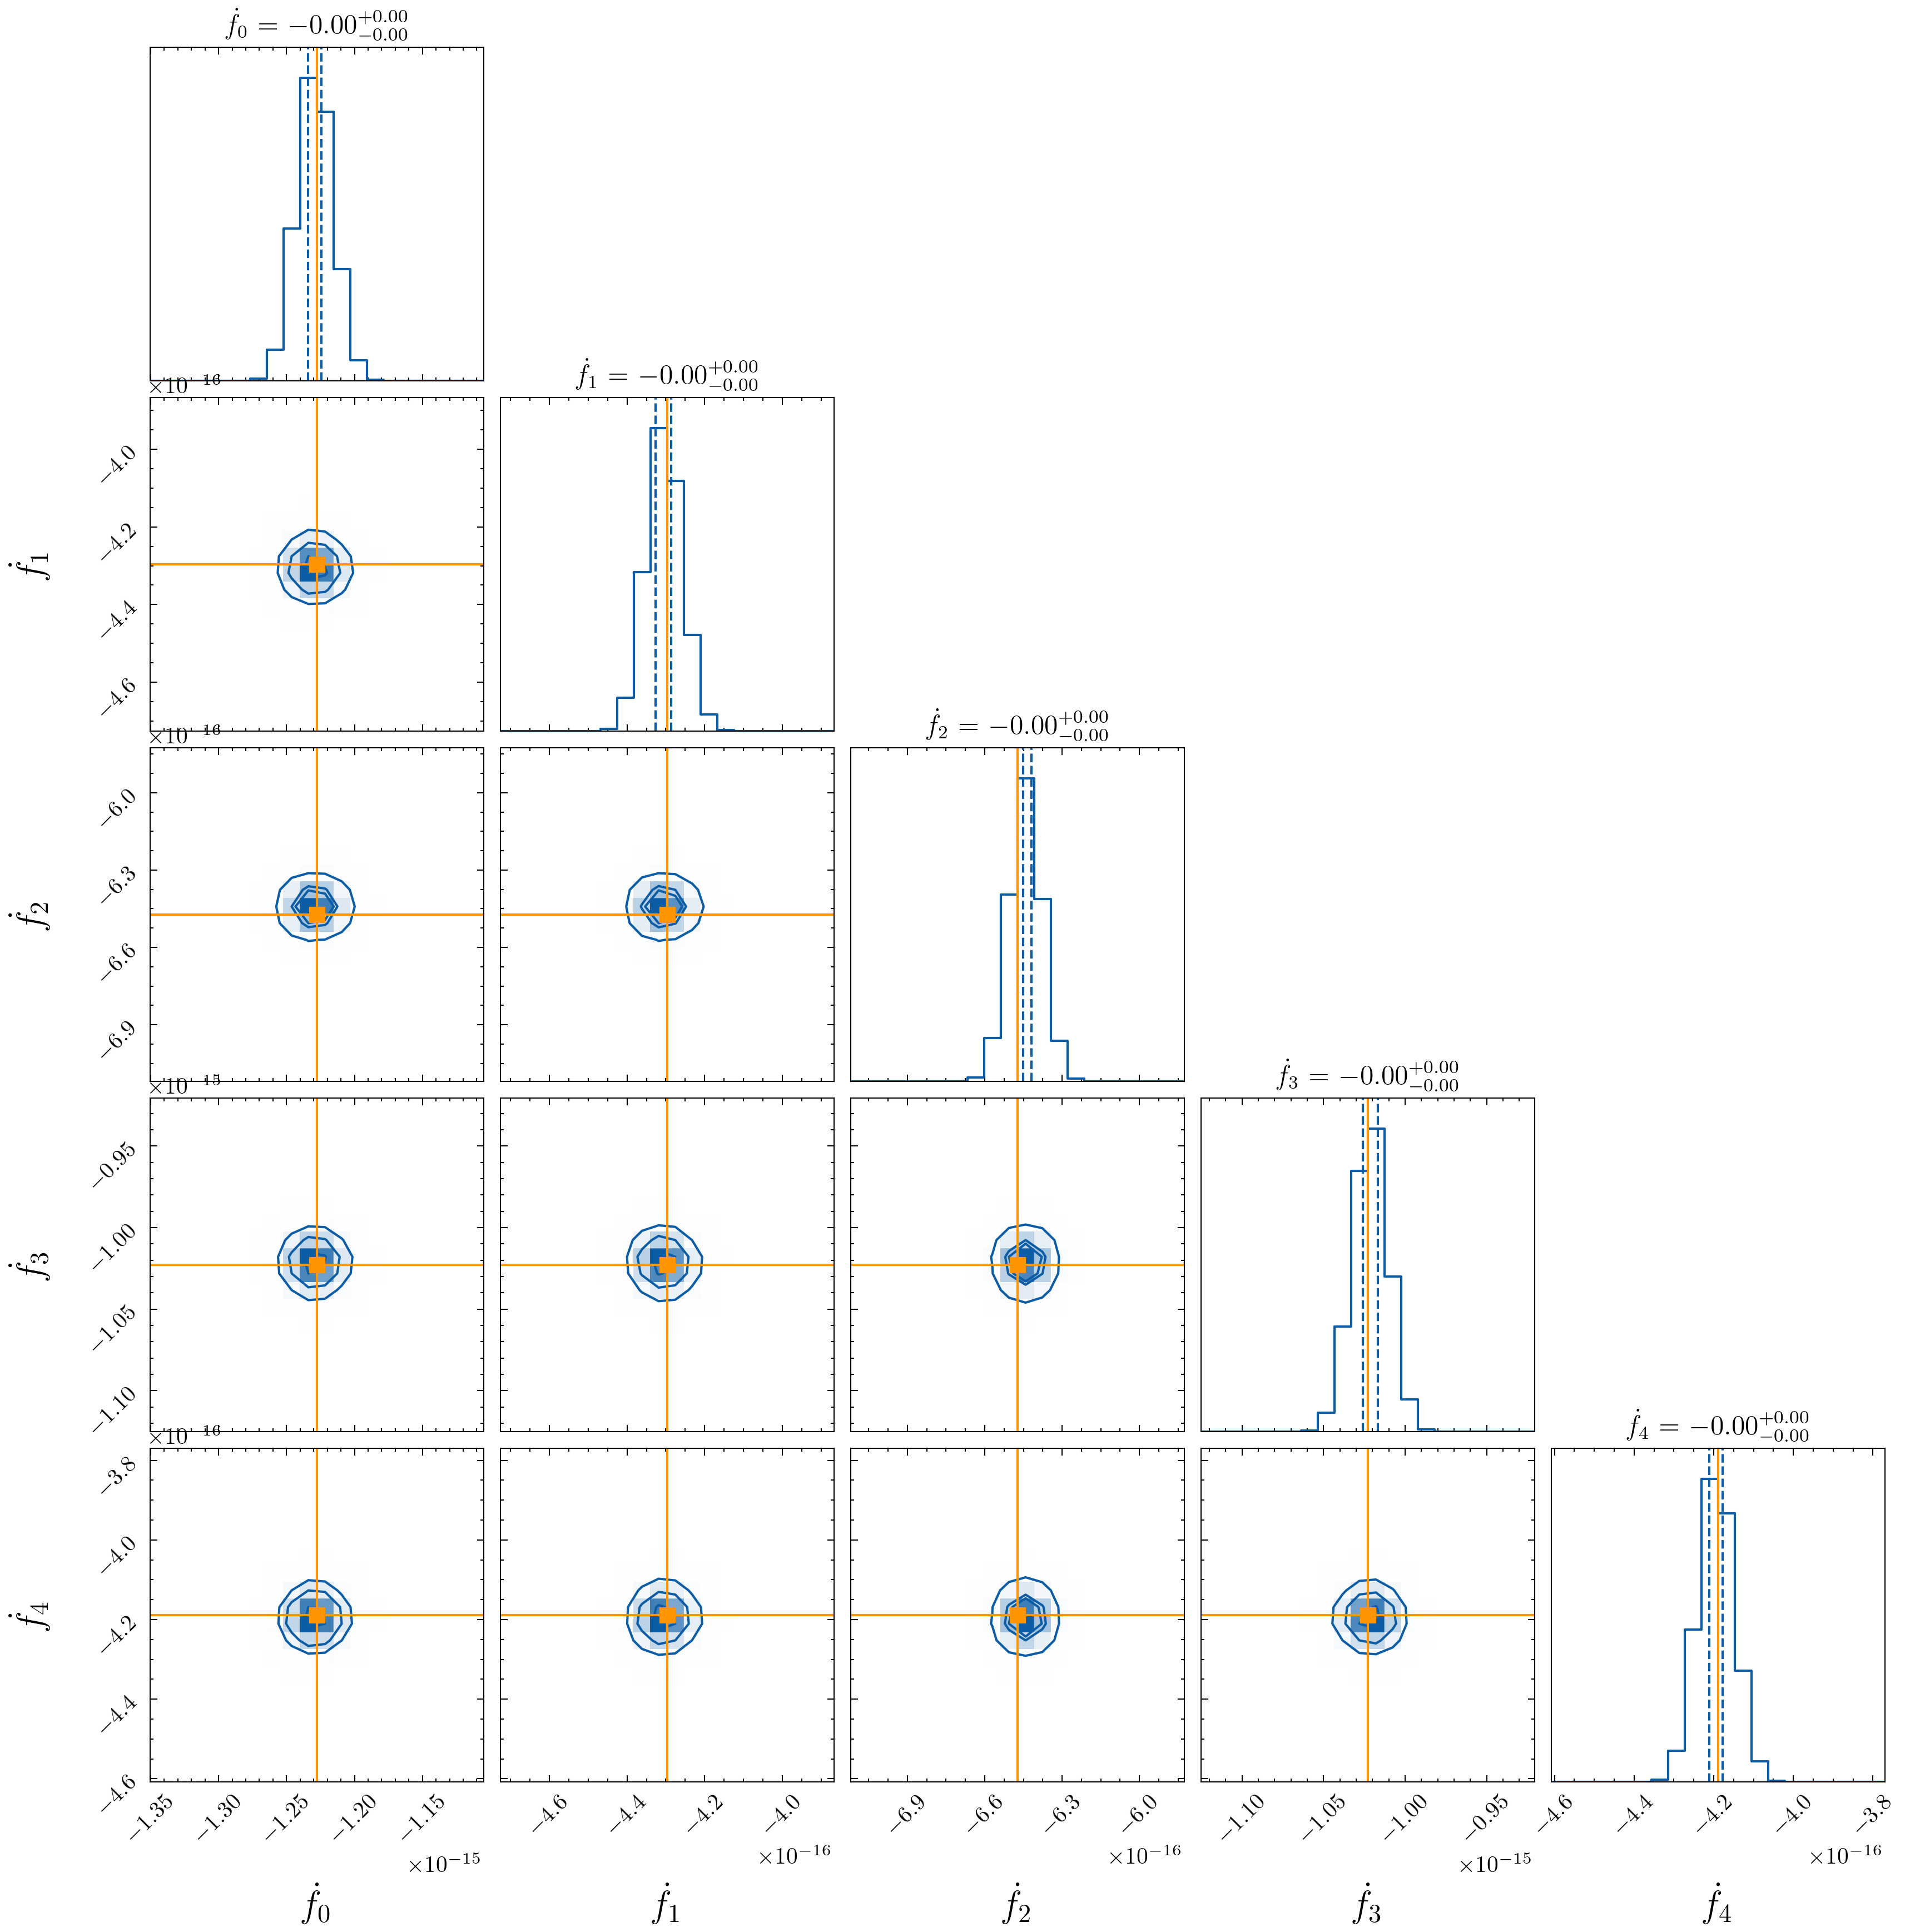
\includegraphics[width=0.85\textwidth,height=0.85\textwidth]{images/1237_broad_fdot}
	
	\only<1>{%
		\tikz[overlay,remember picture]
		\node[fill=white,text=black] at ([xshift=1.5cm,yshift=3.5cm]current page.center){Slightly deceptive: very tight priors - to discuss};
	}
	
\end{frame}




	\begin{frame}{}
	
	
	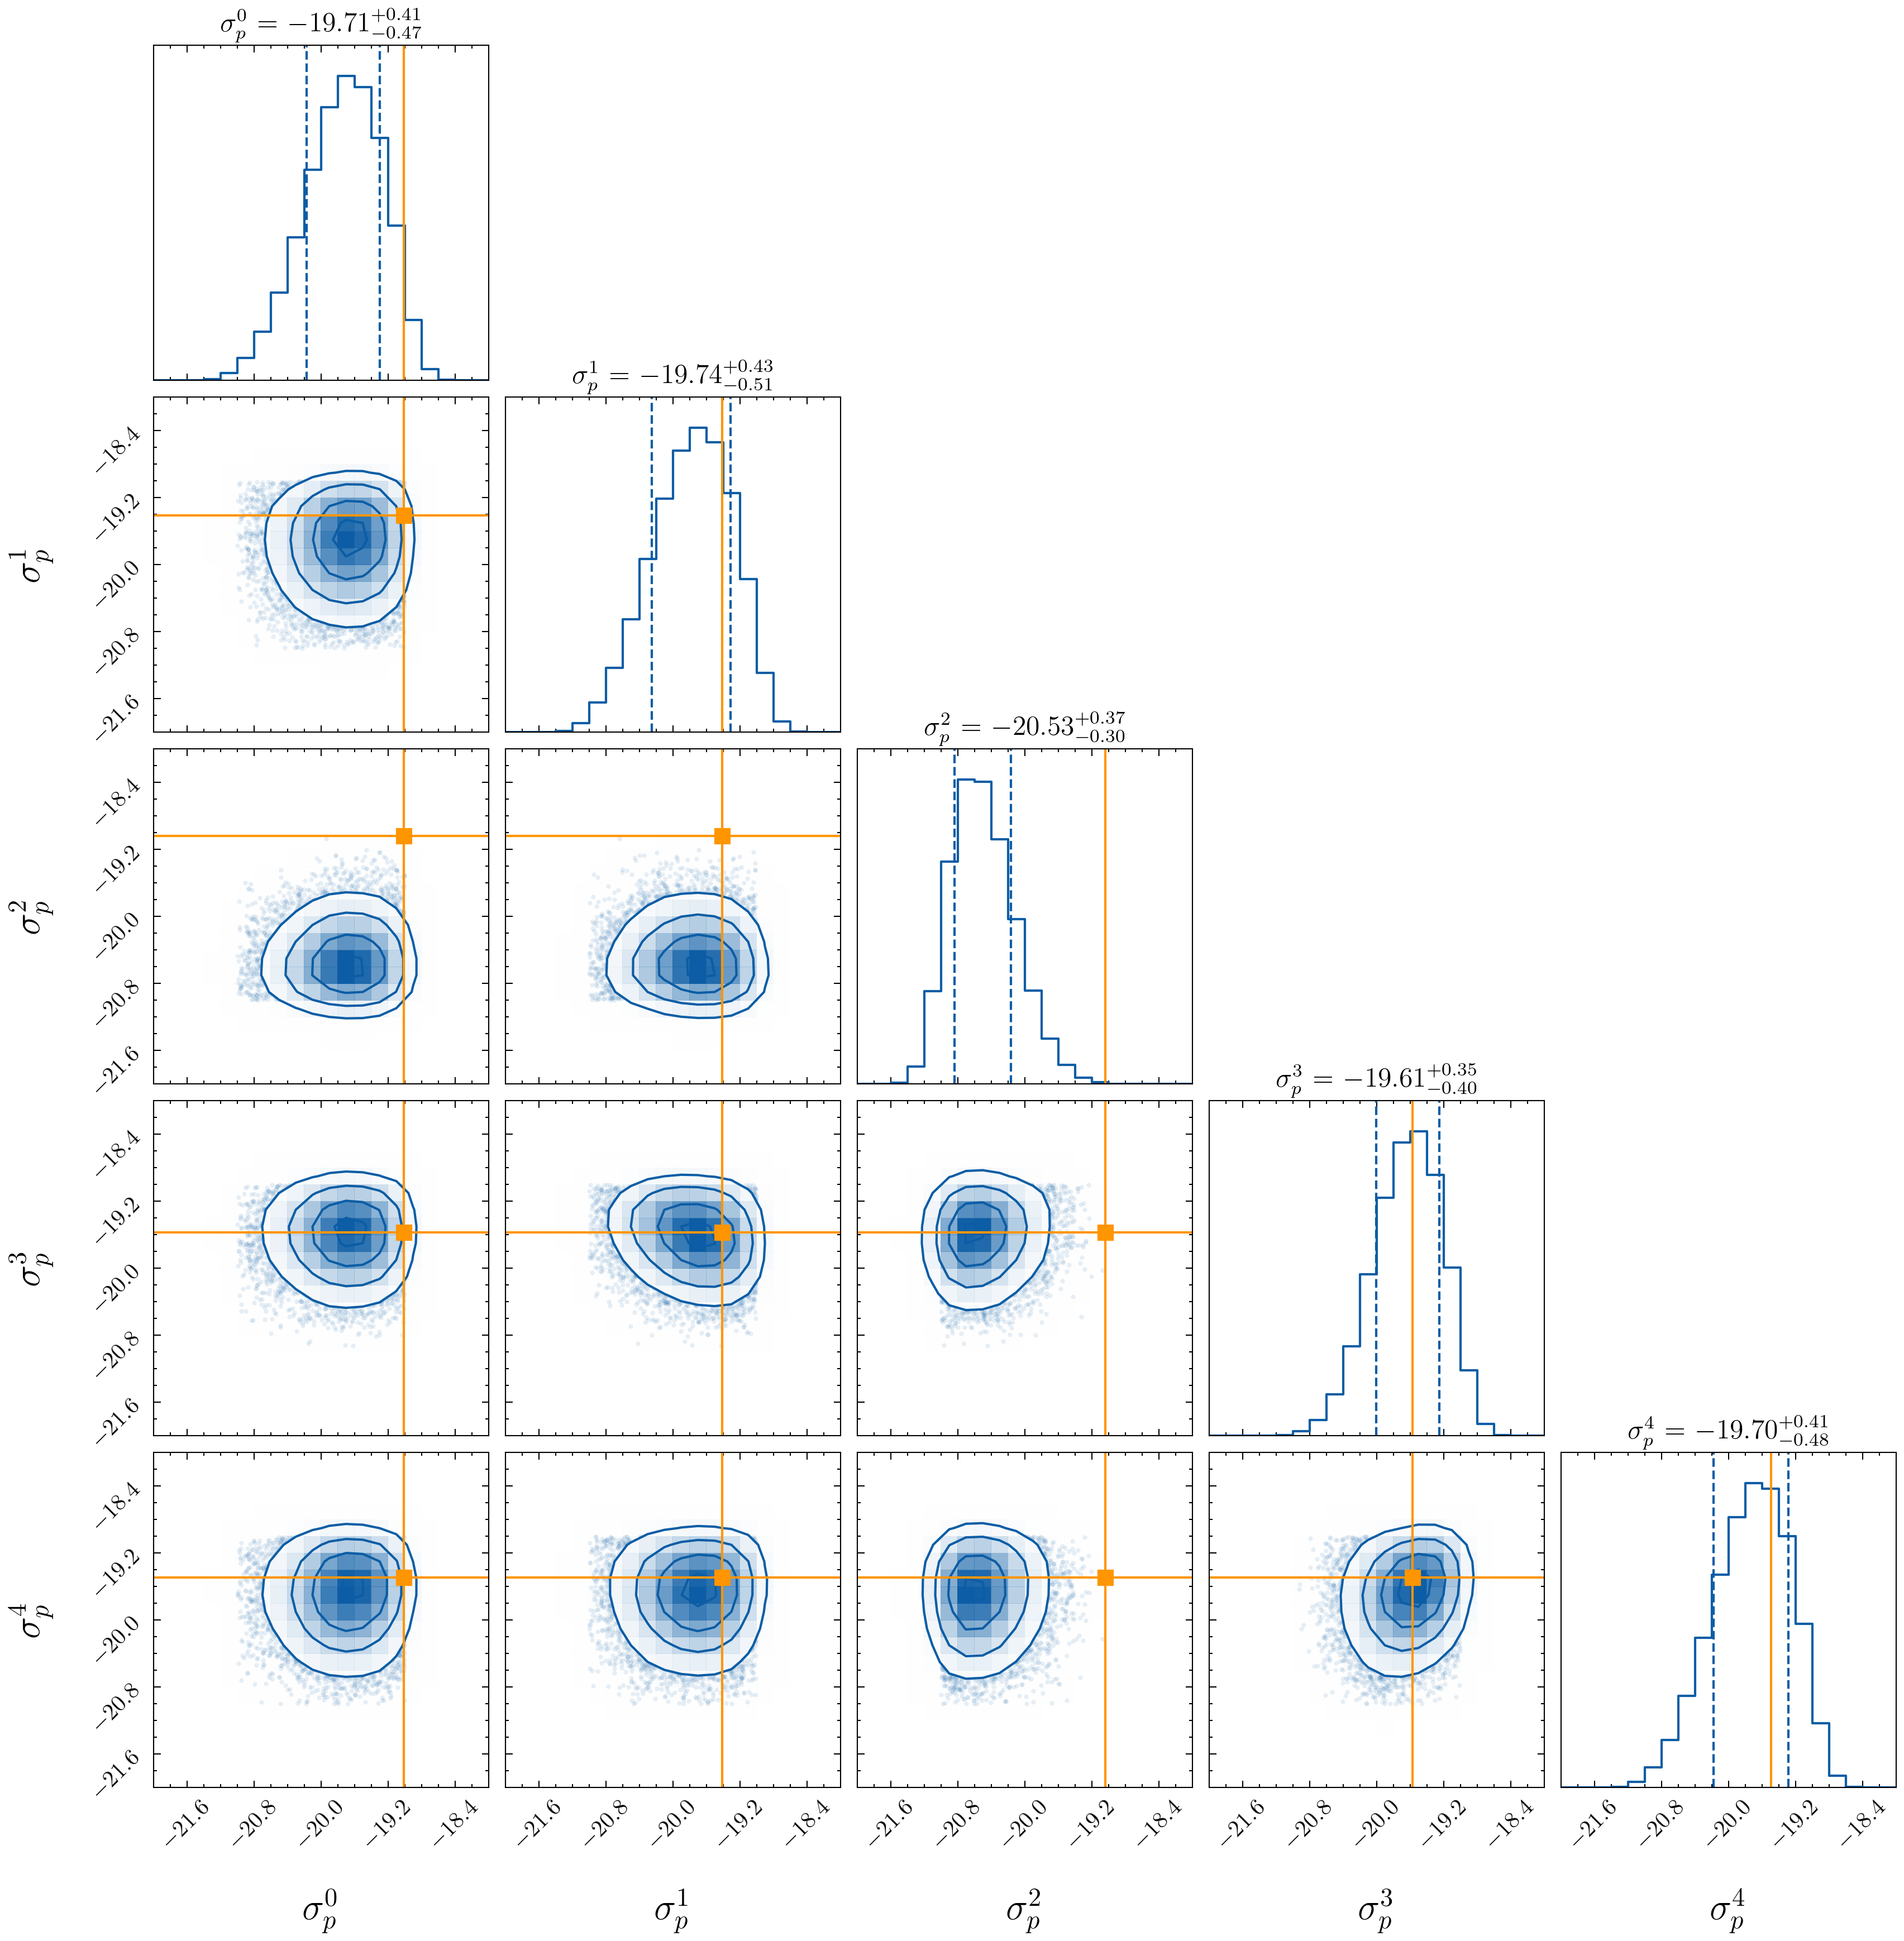
\includegraphics[width=0.85\textwidth,height=0.85\textwidth]{images/1237_broad_sigma_p}
	
	\only<1>{%
		\tikz[overlay,remember picture]
		\node[fill=white,text=black] at ([xshift=1.5cm,yshift=3.5cm]current page.center){LogUniform prior};
	}
		\only<1>{%
		\tikz[overlay,remember picture]
		\node[fill=white,text=black] at ([xshift=1.5cm,yshift=3.0cm]current page.center){Bad: not super accurate};
		
	}
		\only<1>{%
	\tikz[overlay,remember picture]
	\node[fill=white,text=black] at ([xshift=1.9cm,yshift=2.5cm]current page.center){Good: does not impact estimates of $\bar{\theta}_{\rm GW}$};
	
}
\end{frame}





%\begin{frame}{}
%	
%	
%	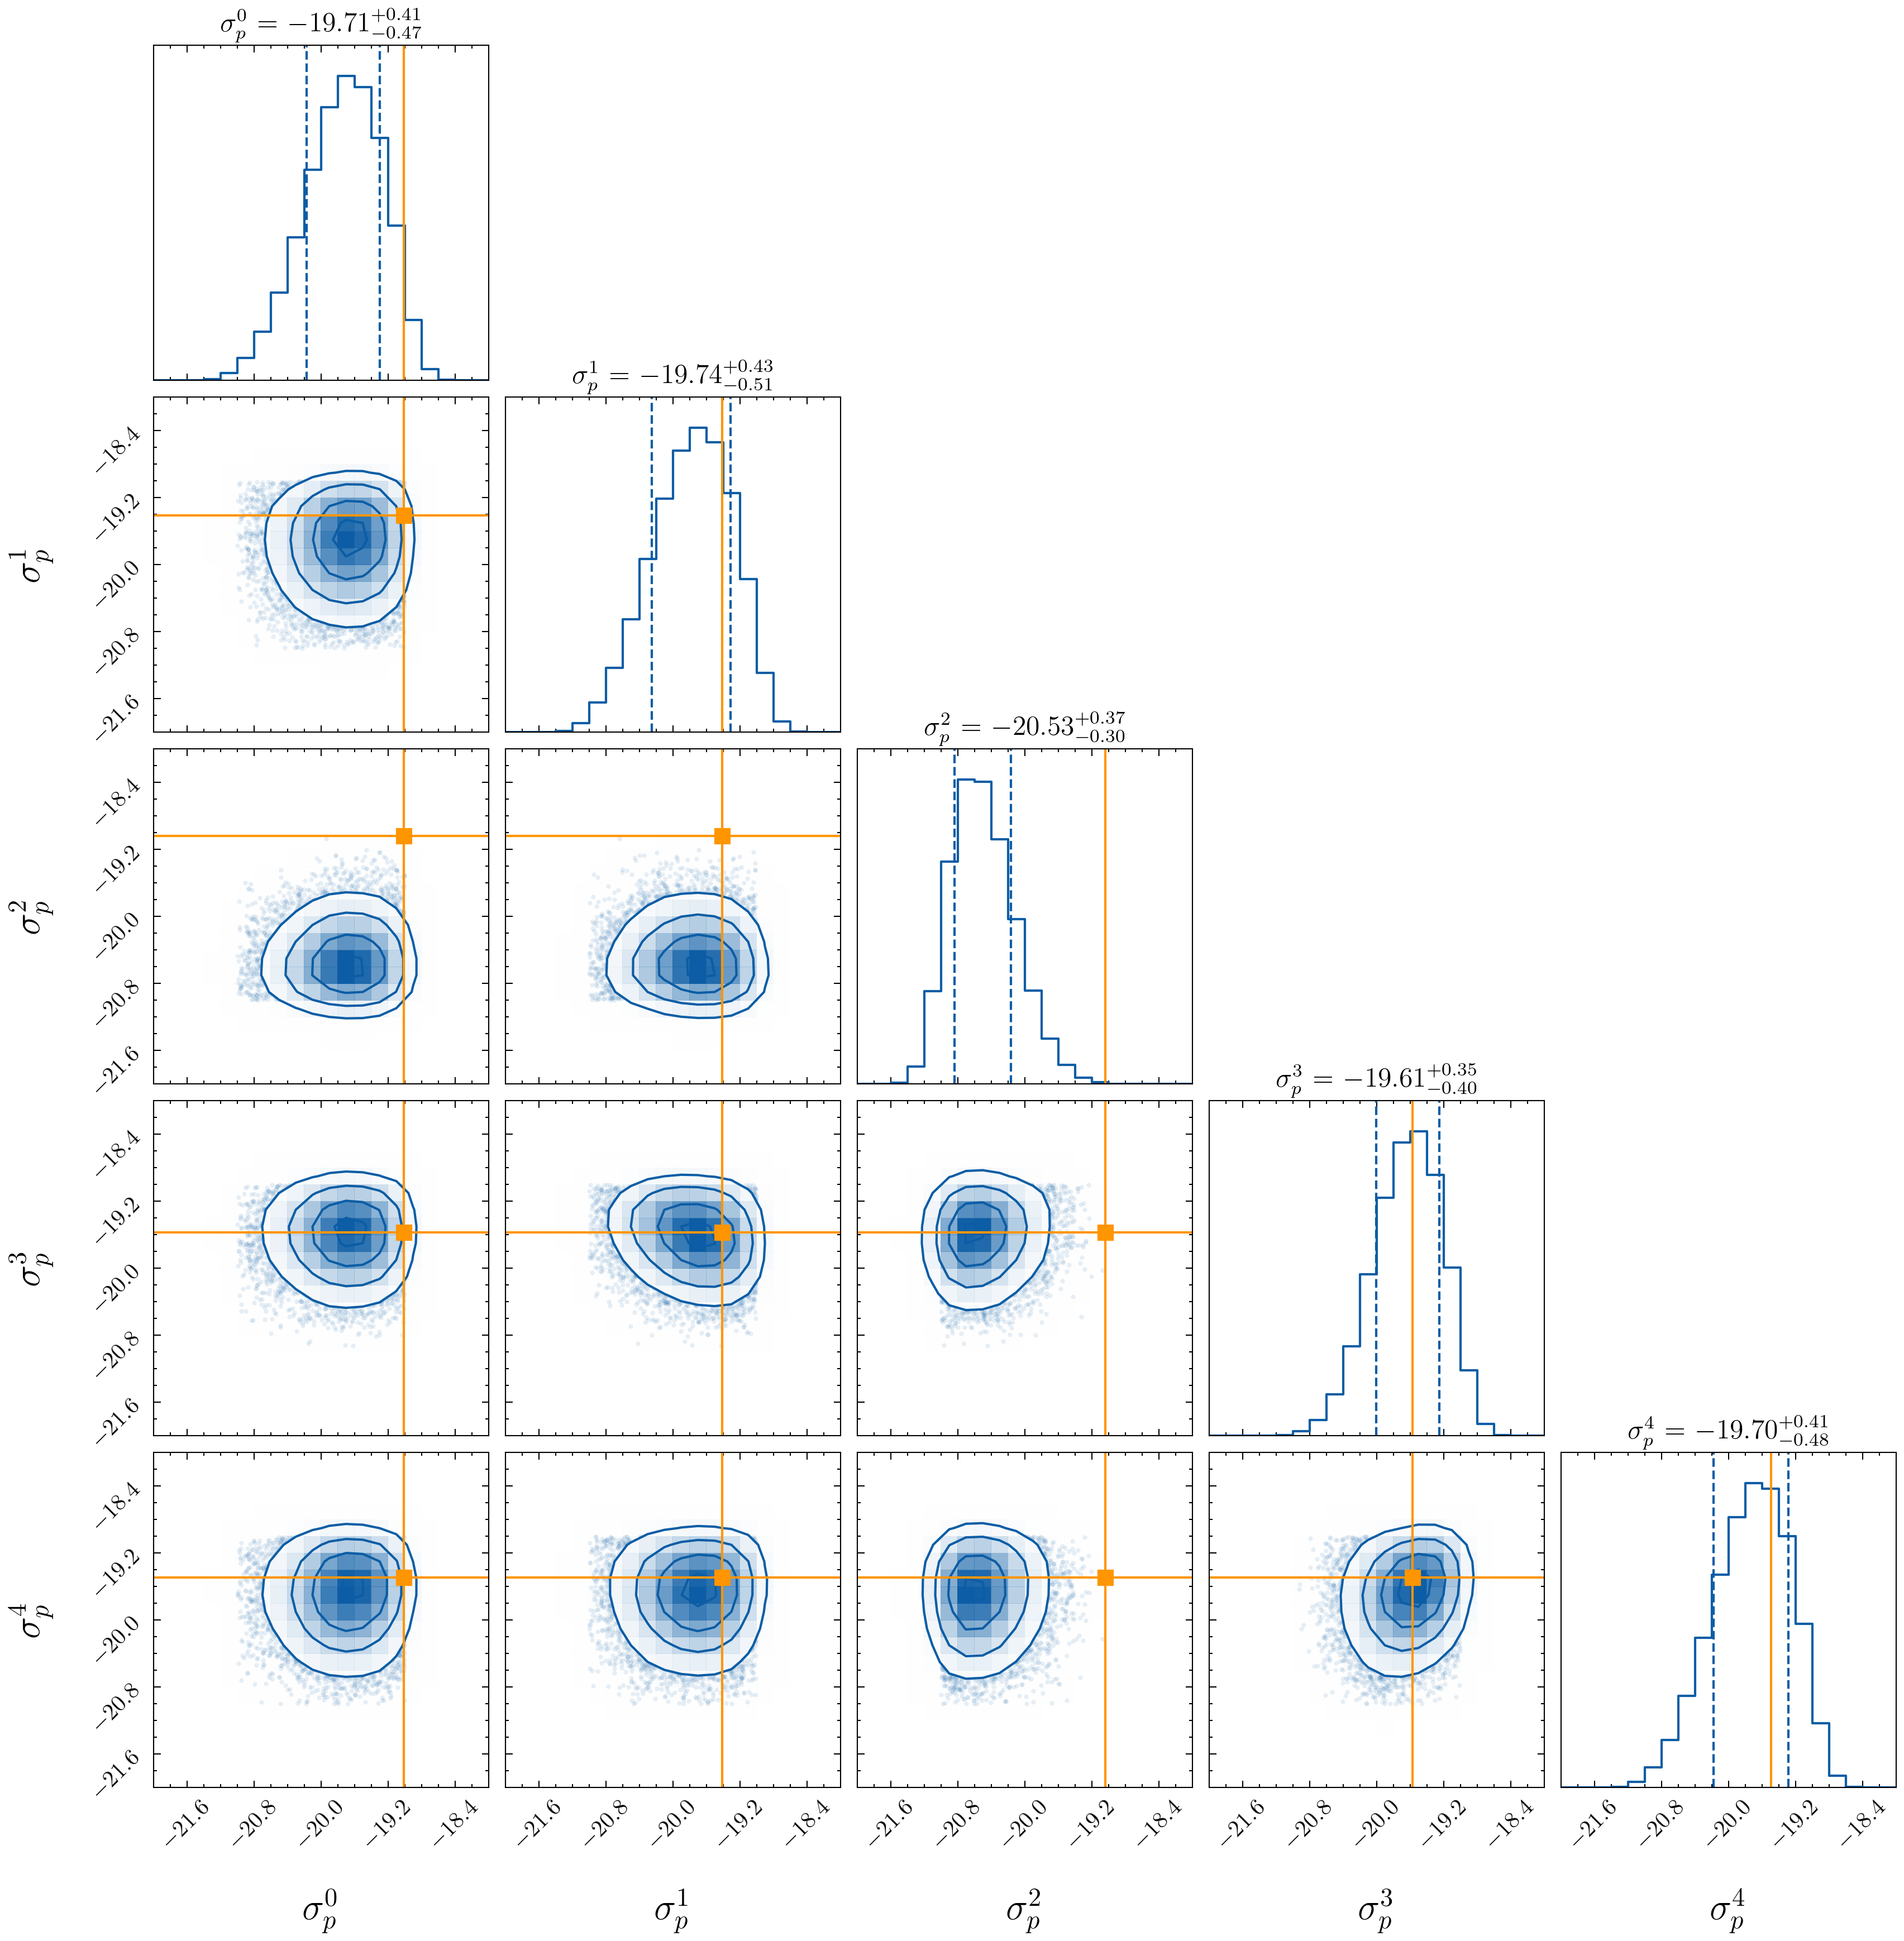
\includegraphics[width=0.85\textwidth,height=0.85\textwidth]{images/1237_broad_sigma_p}
%	
%	\only<1>{%
%		\tikz[overlay,remember picture]
%		\node[fill=white,text=black] at ([xshift=1.5cm,yshift=3.5cm]current page.center){LogUniform prior};
%	}
%\end{frame}





\begin{frame}
	But what about different realisations of a) measurement noise and b) process noise? 
	
	

\end{frame}



	\begin{frame}[label={first_slide_noise}]
	
	
	\includegraphics[width=0.85\textwidth,height=0.85\textwidth]{images/stacked_GW_plot}
	\only<1>{%
		\tikz[overlay,remember picture]
		\node[fill=white,text=black] at ([xshift=1.5cm,yshift=3.5cm]current page.center){As Slide \ref{first_slide}, 5 noise realisations};
	}

\end{frame}




	\begin{frame}
	
	
	\includegraphics[width=0.85\textwidth,height=0.85\textwidth]{images/stacked_f_plot}


	
\end{frame}

	\begin{frame}
	
	
	\includegraphics[width=0.85\textwidth,height=0.85\textwidth]{images/stacked_fdto_plot}
	

	
\end{frame}


	\begin{frame}
	
	
	\includegraphics[width=0.85\textwidth,height=0.85\textwidth]{images/stacked_sgima_p_plot}
	
	
	
\end{frame}




\begin{frame}
	How about 100 noise realisations? 
\end{frame}


	\begin{frame}
	
	
	\includegraphics[width=0.32\textwidth,height=0.85\textwidth]{images/parameter_medians}
	\includegraphics[width=0.32\textwidth,height=0.85\textwidth]{images/parameter_medians_f}
	\includegraphics[width=0.32\textwidth,height=0.85\textwidth]{images/parameter_medians_fdot}
	
	
	
\end{frame}

	\begin{frame}	
	\centering
	\includegraphics[width=0.34\textwidth,height=0.85\textwidth]{images/parameter_medians_sigma_p}
\end{frame}



\begin{frame}
	Case examples - iota, h 
\end{frame}


\begin{frame}{Bayes ratios}


\includegraphics[width=0.85\textwidth,height=0.85\textwidth]{images/BayesRatioPlot}


\end{frame}


\begin{frame}[standout]
	Backup slides
\end{frame}

\appendix



\begin{frame}{Drop PSR terms from model?}
	\begin{equation}
		f_{\rm measured} = f_{\rm emitted} \, g(\tau; \bar{\theta})
		\label{eq:measureent}
	\end{equation}
	with
	\begin{align}
		g(\tau; \bar{\theta}) 
		& = 1 - \frac{1}{2} \frac{ H_{ij}q^i q^j }{(1 + \bar{n}\cdot \bar{q}) } \left[ \cos(-\Omega \tau +\Phi_0) - \cos(-\Omega \tau +\Phi_0 + \Omega (1 + \bar{n}\cdot \bar{q})  d) \right]
	\end{align}
	
	Generate the fake data using the full expression for $g(\tau; \bar{\theta})$, but use $g'(\tau; \bar{\theta})$ in the Kalman measurement model
	
	\begin{align}
		g'(\tau; \bar{\theta}) 
		& = 1 - \frac{1}{2} \frac{ H_{ij}q^i q^j }{(1 + \bar{n}\cdot \bar{q}) } \left[ \cos(-\Omega \tau +\Phi_0) \right]
	\end{align}
\end{frame}


\begin{frame}{Drop PSR terms from model?}
	
	All likelihood curves for $\bar{\theta}_{\rm GW}$:
	\includegraphics[width=0.9\textwidth,height=0.7\textwidth]{images/all_likelihood_curves_psr}
	
\end{frame}



\begin{frame}
	Full NS search for \alert{all parameters} \newline 
	$\bar{\theta} = [\bar{\theta}_{\rm GW}, \, f_0, \, \dot{f}_0]$ \newline 
	with $h = [10^{-10}, 10^{-12}]$, $\sigma_m = 10^{-11}$ \newline 
	Note: pulsar distance is no longer part of model. $\gamma$ doesn't matter
	

\end{frame}


\begin{frame}
		\includegraphics[width=0.85\textwidth,height=0.85\textwidth]{images/canonical_mixed_result_10}
		\only<1>{%
			\tikz[overlay,remember picture]
			\node[fill=white,text=black] at ([xshift=1.5cm,yshift=3.5cm]current page.center){$h = 10^{-10}$,  $\bar{\theta}_{\rm GW}$};

		}
			\only<1>{%
		\tikz[overlay,remember picture]
		\node[fill=white,text=black] at ([xshift=1.5cm,yshift=2.5cm]current page.center){Note some systematics in $\alpha$, $\psi$};
		
	}
\end{frame}


\begin{frame}
	\includegraphics[width=0.85\textwidth,height=0.85\textwidth]{images/canonical12_result}
	\only<1>{%
		\tikz[overlay,remember picture]
		\node[fill=white,text=black] at ([xshift=1.5cm,yshift=3.5cm]current page.center){$h = 10^{-12}$,$\bar{\theta}_{\rm GW}$};
		
	}
	\only<1>{%
		\tikz[overlay,remember picture]
		\node[fill=white,text=black] at ([xshift=1.5cm,yshift=2.5cm]current page.center){Note $h -\iota$ trade-off};
		
	}


\end{frame}


\begin{frame}
\includegraphics[width=0.85\textwidth,height=0.85\textwidth]{images/canonical12_f_result}
\only<1>{%
	\tikz[overlay,remember picture]
	\node[fill=white,text=black] at ([xshift=1.5cm,yshift=3.5cm]current page.center){$h = 10^{-12}$, $f_0$, all (47) PSRs};
	
}

\end{frame}


\begin{frame}
	\includegraphics[width=0.85\textwidth,height=0.85\textwidth]{images/canonical12_fdot_result}
	\only<1>{%
		\tikz[overlay,remember picture]
		\node[fill=white,text=black] at ([xshift=1.5cm,yshift=3.5cm]current page.center){$h = 10^{-12}$, $\dot{f}_0$, all (47) PSRs};
		
	}
\end{frame}





\begin{frame}
	Next steps:
	\begin{itemize}
		\item Bayes factors vs. strain (currently running)
		\item Process noise $\sigma_p$ (next slides)
		\item $[h, \iota] \rightarrow [h_{+}, h_{\times}]$  (discussed, easy, helpful?)
		\item Can we add PSR terms back in? Do we need to?
		\item Robustness for different $\bar{\theta}_{\rm GW}$ (overkill? canonical example sufficient?)
	\end{itemize}
\end{frame}


\begin{frame}{Setting the process noise}
	
	
Timing noise model of \href{https://arxiv.org/abs/1010.4794}{Shannon \& Cordes, 2010}
\begin{eqnarray}
 \ln \sigma_p^{\rm TOA} [\mu s] = \ln \alert{C} + \alert{\alpha} \ln \nu [s^{-1}] + \alert{\beta} \ln \dot{\nu} [10^{-15} s^{-2}] + \alert{\gamma} \ln T [years]
\end{eqnarray}

For MSP, $\ln C \sim -20$, $\alpha \sim 1$, $\beta\sim2$, $\gamma \sim 2.4$

Taking $T = 1$ week, for our synthetic NANOGrav pulsars this puts:	 $$\sigma_p^{\rm TOA}  [s] \sim (10^{-19}, 10^{-17}, 10^{-13}) \, \, , \text{(min/median/max)}$$ 

Relate to frequency:
$$ \sigma_p^{\rm f} [Hz] = f \, \frac{\sigma_p^{\rm TOA}}{T}  \sim (10^{-23}, 10^{-21}, 10^{-16}) \, \, , \text{(min/median/max)}$$

Could hit float epsilon issues here... may need to scale state evolution equations, similar to heterodyning the measured data...

\end{frame}




\begin{frame}{Rescaling to avoid float issues}
	State evolution equation (Ornstein–Uhlenbeck)
	\begin{eqnarray}
		\frac{df}{dt}= -\gamma [f - f_{\rm EM}(t)] + \dot{f}_{\rm EM} + \xi(t; \sigma_p)
	\end{eqnarray}
i.e. 
		\begin{eqnarray}
		df = a(f,t) dt + \sigma_p dW
	\end{eqnarray}

Can solve numerically via e.g. Euler-Maruyama

Partition interval $[0,T]$ into $N$ intervals, each width $\Delta t = T/N$ 
\begin{eqnarray}
	f_{n+1} = f_{n} + a(f_n, \tau_n) \Delta t + \sigma_p \Delta W_n
\end{eqnarray}
\begin{eqnarray}
		\mathcal{O}(10^2) = \mathcal{O}(10^2) + \mathcal{O}(10^{-15}) \cdot \Delta t  + \mathcal{O}(10^{-20}) \Delta W_n
\end{eqnarray}

Practically: synthetic data (float64) generated with e.g. $\sigma_p = 10^{-19}$ = data with e.g. $\sigma_p = 10^{-20}$ 

	
\end{frame}

\begin{frame}{}
	\includegraphics[width=0.90\textwidth,height=0.60\textwidth]{images/sigma_p_non_hetero}
	
	
\end{frame}


\begin{frame}{}
	Let $f \, ' = f - f_{\rm EM}$
	\begin{align}
		\frac{df \, '}{dt}&= \frac{df}{dt} - \frac{df_{\rm EM}}{dt} \\
		                    &= \frac{df}{dt} - \frac{df_{\rm EM}}{dt} \\
		                    &= - \gamma f \, '  + \xi 
	\end{align}
	Now numerical solution looks like
	\begin{eqnarray}
				\mathcal{O}(10^{-12}) = \mathcal{O}(10^{-13}) \cdot \mathcal{O}(10^{-12}) \cdot \Delta t  + \mathcal{O}(10^{-20})
	\end{eqnarray}
	\begin{eqnarray}
	\mathcal{O}(1) = \mathcal{O}(10^{-13}) \cdot \Delta t  + \mathcal{O}(10^{-8})
\end{eqnarray}


	
	Practically: synthetic data (float64) generated with e.g. $\sigma_p = 10^{-19}$ $\neq$ data with e.g. $\sigma_p = 10^{-20}$ 
	
	
\end{frame}

\begin{frame}{}
	\includegraphics[width=0.90\textwidth,height=0.60\textwidth]{images/sigma_p_hetero}
	
\end{frame}




\begin{frame}{Heterodyne state and measurement?}
	
	\begin{itemize}
		\item Heterodyne the state: $f \, ' = f - f_{\rm EM}$ 
		\item Heterodyne the measurement: $f \, '_{\rm M}  = f_{\rm M} - f^{\, *}_{\rm EM}$ 
	\end{itemize}
	
	$f_{\rm EM}$ is the exact, true solution parametrised by the unknowns $f_0, \dot{f}_0$
	
	 $f^{\, *}_{\rm EM}$ is a guess based on the pulsar ephemeris. 
	 
	 For our case where we have synthetic data we can set $f_{\rm EM} = f^{\, *}_{\rm EM}$, but obviously not true generally - we are trying to estimate $f_{\rm EM}$!
	
	We can then write the measurement equation as
	\begin{eqnarray}
		f_{\rm M} = (1 - X)f + N_{\rm G} 
	\end{eqnarray}
\begin{eqnarray}
	f \, '_{\rm M} = (1 - X)f \, ' - X f_{\rm EM} + \alert{(f_{\rm EM} - f^{\, *}_{\rm EM})} +  N_{\rm G}
\end{eqnarray}
	
	\begin{itemize}
		\item Linear \checkmark (control vector has shifted from state equation to measurement equation)
		\item Scales: $\mathcal{O}(h) = \mathcal{O}(10^{-12}) - \mathcal{O}(h)\cdot\mathcal{O}(10^2) + \alert{\mathcal{O}(0)} + \mathcal{O}(10^{-11})$ \checkmark
	\end{itemize}
	
	
\end{frame}



\begin{frame}{}
	
Insert corner plot here
	
	
\end{frame}




\begin{frame}[fragile]{Where did $\sigma_m$ value come from?}
The measurement noise is

$$ \sigma_m = f \frac{\sigma_{\rm TOA}}{\rm cadence}$$

So for a MSP ( $f \sim 100 Hz$) observed with a weekly cadence and $\sigma_{\rm TOA} \sim 1 \mu$s:


$$\sigma_m \sim 1.6 \times 10^{-10}$$

The very best pulsars might have $\sigma_{\rm TOA} \sim 10$ ns:

$$\sigma_m \sim 1.6 \times 10^{-12}$$
\end{frame}







\begin{frame}{$\gamma$ likelihood}
	\includegraphics[width=0.8\textwidth,height=0.8\textwidth]{images/likelihood_gamma_1}
\end{frame}


	\begin{frame}{What changed?}
		
		AM: \textit{"What changed such that now everything works?"}
		
		\begin{itemize}
			\item Dropping PSR terms to smooth likelihoods
			\item \textit{Increasing} measurement noise  
			\item Don't need too many live points
			\begin{itemize}
				\item $n_{live} > $ number of parameters 
				\item $n_{live} \times \frac{\rm mode \, volume}{\rm prior \, volume} > 1 $ i.e. at least 1 live point per mode
				\item Runtime scales $\mathcal{O}(n_{live})$
				\item Posterior/Evidence uncertainties scale as $\mathcal{O}(1 / \sqrt{n_{live}})$
			\end{itemize}
			
			\item Non-default Bilby sampler settings 
			\begin{itemize}
				\item e.g. docs recommend `sample=act-walk`or `sample=acceptance-walk`
				\item More success with `sample=rwalk-dynesty` (not `sample=rwalk` which is the Bilby implementation)
				\item bound = multi(dynesty), not the Bilby version 
			\end{itemize}
		\item Be mindful of float errors - Python/Numpy/Bilby NaNs get propagated, rather than error e.g. Fortran.
		\end{itemize}
	

	
\end{frame}



\begin{frame}{More likelihood curves}
	
	Example: $\mathcal{L}(\delta)$
	
\includegraphics[width=0.7\textwidth,height=0.6\textwidth]{images/likelihood_delta_1}
	
	
\end{frame}

\begin{frame}{}
	
	Example: $\mathcal{L}(\delta)$, zoomed 1
	
	\includegraphics[width=0.7\textwidth,height=0.6\textwidth]{images/likelihood_delta_2}
	
	
\end{frame}


\begin{frame}{}
	
	Example: $\mathcal{L}(\delta)$, zoomed 2
	
	\includegraphics[width=0.7\textwidth,height=0.6\textwidth]{images/likelihood_delta_3}
	
	
\end{frame}


\begin{frame}{}
	
	Example: $\mathcal{L}(\omega)$
	
	\includegraphics[width=0.7\textwidth,height=0.6\textwidth]{images/likelihood_omega_1}

	
\end{frame}


\begin{frame}{}
	
	Example: $\mathcal{L}(\omega)$, zoomed 1
	
	\includegraphics[width=0.7\textwidth,height=0.6\textwidth]{images/likelihood_omega_2}
	
	
\end{frame}


\begin{frame}{}
	
	Example: $\mathcal{L}(\omega)$, zoomed 2
	
	\includegraphics[width=0.7\textwidth,height=0.6\textwidth]{images/likelihood_omega_3}
	
	
\end{frame}






\begin{frame}{}
	
		\begin{itemize}
		\item \alert{Problem} = overly narrow,biased posteriors
		\item Cause: noisy, likelihoods which are "locally Gaussian". Sampling gets stuck in a local optima and infers posteriors widths based on that optima. 

%		\end{itemize}
	\end{itemize}
	
	
	
\end{frame}


\begin{frame}{Potential solutions to noisy likelihoods}

	
	\begin{enumerate}
		\item Better settings for sampler? E.g. more live points (how many?), massively parallel, optimized likelihood evaluations,...
		\item Maximum likelihood / loss optimisation? 
		\item Drop PSR terms from model?
		\item MCMC at higher temperatures (trades off evidence..., less efficient	)
		\item other...?
	\end{enumerate}
	
	
\end{frame}








%	\begin{frame}{}
	%
	%Numerical weather and climate modelling 
	%
	%        \begin{itemize}
		%	        \item Reduced precision floats + stochastic rounding
		%	        \item Automatic Differentiation
		%        \end{itemize}
	%    
	%    \alert{Open call for collaboration!}
	%    
	%    
	%	\end{frame}



	
\end{document}